\chapter{회전, 스피너, 그리고 색 대칭}

\section{군으로서의 회전}

공간의 회전은 대칭이며, 여러 종류의 대상에 작용한다. 회전은 강체, 속도 벡터, 벡터장, 양자 상태에 작용한다. 보통의 벡터는 변환을 직접 그림으로 나타낼 수 있으므로 가장 간단한 출발점이다.

회전은 합성할 수도 있다. 물체를 한 축을 중심으로 한 각도만큼 회전시킨 다음, 두 번째 축을 중심으로 다른 각도만큼 회전시킨다고 하자. 최종 방향은 어떤 세 번째 축을 중심으로 어떤 세 번째 각도만큼 회전한 결과와 같다. 따라서 두 회전의 곱도 하나의 회전이다.

이 곱은 두 축 벡터를 더하는 것이 아니라 변환에 대한 연산이다. 첫 번째 회전은 두 번째 회전이 작용하는 대상을 바꾼다. \(R_1\)를 먼저 하고 \(R_2\)를 다음에 하면, 합성 연산은 \(R_2R_1\)로 쓴다. 축과 각도를 구하기가 불편할 수는 있지만, 이 합성 연산 자체는 어떤 \(R_3\)이다. 합성에 대해 닫혀 있다는 점은 회전을 단순한 기하학적 운동의 목록이 아니라 군으로 보아야 하는 첫 번째 이유다. 다만 \(R_3\)의 축과 각도를 구하기는 불편할 수 있다.

먼저 회전 하나를 기하학적으로 기술해 보자. 회전축을 따라가는 단위 벡터 \(\hat{\boldsymbol n}\)와 각도 \(\theta\)을 정한다. 오른손 규약을 채택하자. 왼손 방향으로 \(\theta\)만큼 회전하는 것은 오른손 방향으로 \(-\theta\)만큼 회전하거나 \(-\hat{\boldsymbol n}\)을 축으로 오른손 방향으로 회전하는 것으로 똑같이 나타낼 수 있다.

\begin{figure}[htbp]
\centering
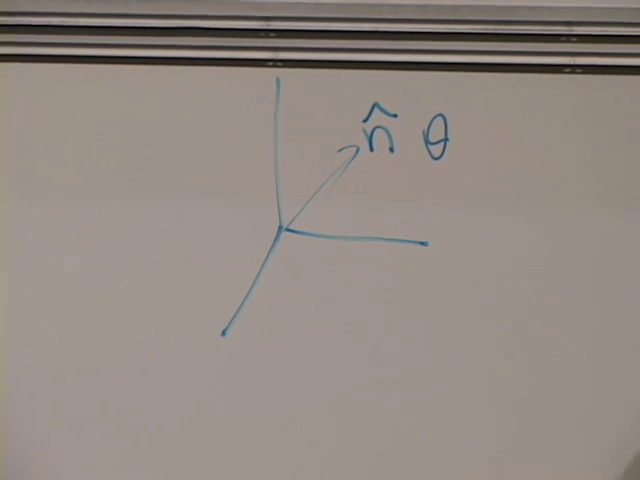
\includegraphics[width=0.58\textwidth]{lecture_03_figure_02.png}
\caption{회전축 \(\hat{\boldsymbol n}\)과 각도 \(\theta\)이 공간 회전을 정한다.}
\lectureframe{00:02:34}
\end{figure}

단위 구면 위의 방향은 경도와 위도처럼 두 매개변수로 정할 수 있다. 그 방향을 축으로 하는 회전각이 세 번째 매개변수다. 따라서 회전은 세 매개변수로 이루어진 족을 이룬다. 각도가 \(2\pi\)만큼 차이 날 때 생기는 전역적 동일시 문제는 아직 고려하지 않겠다. 여기서는 국소적인 매개변수의 개수가 중요하다.

축-각도 표현에는 중복이 있다. 축의 방향과 각도의 부호를 함께 뒤집어도 같은 연산이고, 충분히 큰 각도는 한 바퀴를 기준으로 줄일 수 있다. 그래도 항등원 근처에서 회전이 연속적으로 변하는 매개변수 세 개를 가진다는 사실은 달라지지 않는다. 이 국소적인 개수는 나중에 행렬 표현의 독립 매개변수 개수와 대응시킬 것이다.

이제 군의 성질을 차례로 확인할 수 있다:
\begin{enumerate}
\item \emph{닫힘.} 회전을 연이어 두 번 하면 또 다른 회전이 된다.
\item \emph{항등원.} 아무것도 하지 않는 것이 항등 회전이다.
\item \emph{역원.} \(\hat{\boldsymbol n}\)을 축으로 \(\theta\)만큼 회전한 것은 같은 축을 중심으로 \(-\theta\)만큼 회전하면 되돌릴 수 있다.
\item \emph{결합법칙.} 회전 세 번을 연이어 하면 다음이 성립한다.
\[
(R_1R_2)R_3=R_1(R_2R_3).
\]
\end{enumerate}

회전은 교환법칙을 따르지 않는다. \(x\)축을 중심으로 회전한 다음 \(y\)축을 중심으로 회전하면, 일반적으로 같은 두 연산을 역순으로 했을 때와 방향이 달라진다:
\begin{equation}
R_x(\alpha)R_y(\beta)\ne R_y(\beta)R_x(\alpha).
\end{equation}
두 각도가 모두 매우 작으면 차이는 2차항부터 나타나므로 무한소 회전은 거의 교환하는 것처럼 보일 수 있다. 그렇지만 전체 군은 비가환군이다.

어떤 방정식도 쓰지 않고 비가환성을 확인할 수 있다. 책이나 상자를 가져와 한 면을 앞면으로 표시한 뒤, \(x\)축을 중심으로 90도 회전하고 이어서 \(y\)축을 중심으로 90도 회전해 보자. 처음 방향으로 되돌아가 회전 순서를 바꾸어도 같은 동작을 해 보자. 표시한 면은 서로 다른 방향을 향하게 된다. 각도가 작으면 차이를 알아보기 어렵지만, 차이가 사라진 것은 아니다. 두 작은 각도의 곱에서 시작한다.

\begin{classroomqa}
\audiencequestion{이 회전들은 동시에가 아니라 차례로 하는 건가요?\lecturetimestamp{00:04:45}}
\lecturerresponse{그렇습니다. 군의 곱셈은 한 연산을 한 다음 다른 연산을 하는 것을 뜻합니다. 바로 이 연속된 회전들의 순서 때문에 교환법칙이 성립하지 않을 수 있습니다.}
\end{classroomqa}

이것이 우리가 처음 만나는 비가환군이다. 여기서 궁극적으로 다룰 대상은 보통 물체의 색이 아니라 쿼크의 빨강, 초록, 파랑 색 상태다. 이는 세 상태를 가진 내부 계이며, 흥미로운 변환은 세 색을 서로 섞는다. 보통의 회전은 연속군이 행렬을 통해 작용하는 방식을 보여 주는 친숙한 본보기다.

군 자체는 추상적이다. 물리학에서 군을 쓰려면 어떤 대상에 작용하는지 말해야 한다. {표현}은 각 군 원소에 연산자나 행렬을 대응시켜 군 원소의 곱셈이 대응하는 행렬들의 곱셈으로 재현되도록 한다. 서로 다른 물리적 대상은 같은 군의 서로 다른 표현을 가질 수 있다. 벡터, 스핀 1 상태, 스핀 1/2 상태가 세 가지 예가 될 것이다.

\section{3차원 벡터 표현}

보통의 벡터 성분을 다음과 같이 쓰자.
\begin{equation}
\boldsymbol V=(V_x,V_y,V_z),\qquad V_i,\quad i=1,2,3.
\end{equation}
좌표축을 고정한 채 물리적 벡터를 회전시킬 수도 있고, 벡터를 고정한 채 좌표축을 회전시킬 수도 있다. 두 방식의 규약은 다르지만 어느 쪽이든 성분은 \(3\times3\) 행렬에 의해 서로 섞인다. 축-각도 쌍 \((\hat{\boldsymbol n},\theta)\)마다 다음과 같이 쓰자.
\begin{equation}
V_i'=R_{ij}(\hat{\boldsymbol n},\theta)V_j,
\label{eq:l3-vector-rotation}
\end{equation}
여기서 반복된 첨자는 합산한다.

반복된 첨자 \(j\)는 더미 첨자다. 식~\eqref{eq:l3-vector-rotation}은 각 출력 성분 \(i\)에 대해 다음을 뜻한다.
\begin{equation}
V_i'=R_{i1}V_1+R_{i2}V_2+R_{i3}V_3
\end{equation}
자유 첨자 \(i\)는 계산할 성분을 표시하고, 반복된 첨자 \(j\)는 합산하며 식을 바꾸지 않고 이름을 바꿀 수 있다. 이 두 역할을 구분하면 길이 보존 논증에서 발생하는 대부분의 첨자 오류를 막을 수 있다.

\begin{figure}[htbp]
\centering
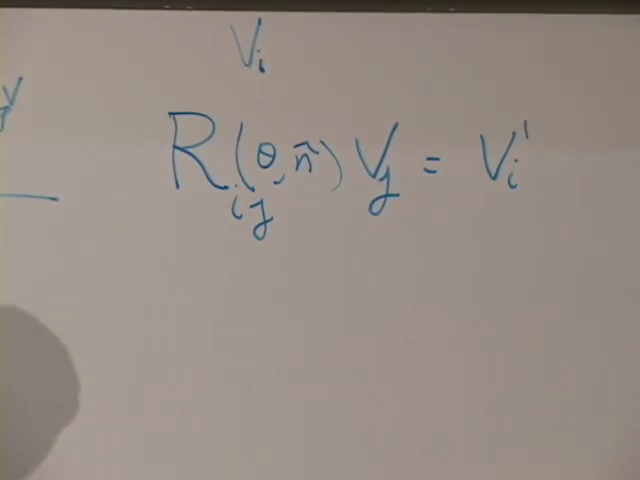
\includegraphics[width=0.68\textwidth]{lecture_03_figure_03.png}
\caption{회전 행렬은 원래 벡터 성분을 회전된 벡터 성분으로 사상한다.}
\lectureframe{00:07:41}
\end{figure}

참된 회전은 길이를 보존한다. 우선 \(V_i\)와 \(R_{ij}\)가 모두 실수이므로 다음이 성립한다.
\begin{equation}
V_i'V_i'=V_iV_i
\end{equation}
이는 모든 벡터에 대해 성립한다. 행렬 조건을 드러내기 위해 같은 변환을 더미 첨자를 달리해 쓰면 다음과 같다.
\begin{equation}
V_i'=R_{ij}V_j,\qquad V_i'=R_{ik}V_k.
\end{equation}
\(i\)에 대해 곱한 뒤 합하면 다음을 얻는다.
\begin{align}
V_i'V_i'
 &=R_{ij}V_jR_{ik}V_k\\
 &=R_{ij}R_{ik}V_jV_k.
\end{align}
이는 \(V_jV_j\)와 같아야 한다. 이 등식이 \(V\)의 모든 값에 대해 성립하려면 다음 조건이 필요하다.
\begin{equation}
R_{ij}R_{ik}=\delta_{jk}.
\label{eq:l3-orthogonality-index}
\end{equation}
행렬 표기법으로는
\begin{equation}
R^TR=\boldsymbol 1,
\label{eq:l3-orthogonal}
\end{equation}
따라서
\begin{equation}
R^{-1}=R^T.
\end{equation}
전치하면 행과 열이 서로 바뀐다.

계수가 왜 \(\delta_{jk}\)여야 할까? 크로네커 델타는 합산에서 \(j=k\)을 지정한다.
\begin{equation}
\delta_{jk}V_jV_k=V_1^2+V_2^2+V_3^2.
\end{equation}
\(R_{ij}R_{ik}\)가 \(\delta_{jk}\)와 다르면 어떤 방향이나 교차항 \(V_jV_k\)가 길이를 바꾸게 된다. 등식은 임의로 택한 한 벡터만이 아니라 가능한 모든 벡터에 대해 성립해야 하므로 행렬의 계수 자체가 항등행렬이어야 한다.

식~\eqref{eq:l3-orthogonal}은 이 실수 행렬 표현을 정의하는 직교 조건이다. 행렬을 곱하면 공간 회전의 곱셈표가 재현된다. 회전군의 표현이 이것뿐인 것은 아니다. 단지 가장 쉽게 시각화할 수 있는 표현이다.

역원 관계는 즉각적인 기하학적 의미를 갖는다. 새로운 행렬 방정식을 풀지 않고도 행과 열을 맞바꾸면 회전을 되돌릴 수 있다. \(R_1\)와 \(R_2\)가 두 회전을 나타낸다면, \(R_2R_1\)는 두 회전이 차례로 작용한 결과를 나타내며 역시 직교 행렬이다. 따라서 행렬 연산은 기하학적으로 확립한 닫힘, 항등원, 역원, 결합법칙의 구조를 그대로 보존한다.

\section{스핀 1과 벡터 표현}

이 3차원 표현은 양자 상태에도 작용한다. 스핀 1 입자는 다음과 같이 세 가지 스핀 투영값을 갖는다.
\begin{equation}
m=+1,\quad 0,\quad -1.
\end{equation}
따라서 스핀 상태는 확률진폭 세 개로 이루어진 열벡터다. 입자를 회전시키거나 스핀 축을 정의하는 데 쓰는 자기장의 방향을 바꾸면, 회전군의 3차원 표현에 의해 세 진폭이 서로 섞인다.

스핀 상태의 개수는 익숙한 규칙 \(2s+1\)을 따른다. 스핀 0에는 상태가 하나, 스핀 1/2에는 둘, 스핀 1에는 셋, 스핀 3/2에는 넷이 있다. 따라서 상태 벡터의 차원은 스핀에 따라 달라진다. 같은 물리적 회전도 서로 다른 상태 공간에 작용할 때는 크기가 다른 행렬로 표현되어야 한다.

스핀 1 입자에 대해 다음 기저를 택하자.
\begin{equation}
\lvert 1,+1\rangle,qquad
\lvert 1,0\rangle,qquad
\lvert 1,-1\rangle.
\end{equation}
상태는 다음과 같다.
\begin{equation}
\lvert\psi\rangle
=c_{+}\lvert1,+1\rangle+c_0\lvert1,0\rangle+c_{-}\lvert1,-1\rangle.
\end{equation}
장치를 회전시켜도 네 번째 스핀 상태가 생기지는 않는다. 계수 \(c_+,c_0,c_-\)가 서로 섞일 뿐이다. 따라서 이에 대응하는 회전 연산자는 \(3\times3\) 행렬이어야 한다.

스핀 1에서 이 표현은 보통의 공간 벡터와 같은 방식으로 변환된다. 스핀 1 입자를 \emph{벡터 입자}라고 부르는 정확한 의미는 이것이다. 스핀 진폭 세 개와 벡터 성분 세 개가 같은 회전 법칙을 따른다. 양자 상태를 실제 화살표라고 상상할 필요는 없다. 이는 성분들이 서로 섞이는 방식에 관한 설명이다.

이 대응은 우연이 아니다. 3차원 벡터와 스핀 1 상태는 회전군의 동등한 3차원 표현을 따른다. {벡터 입자}라는 말은 그러한 변환 성질을 요약한다. 양자 편광 상태가 입자 안에 숨은 작은 강체 화살표라고 주장하는 것은 아니다.

\section{이산 대칭과 연속 대칭}

스핀 1/2로 넘어가기 전에 두 가지 넓은 종류의 군을 구분하면 도움이 된다. 반사는 간단한 이산적 예다. 항등원이 있고 반사 \(P\)가 있다. 뒤집거나 뒤집지 않거나 둘 중 하나다. 반면 위상 \begin{equation}
e^{i\phi}
\end{equation}는 \(\phi\)에 따라 연속적으로 달라지고, 공간 회전은 축과 각도에 따라 연속적으로 달라진다. 이런 연속군을 Sophus Lie의 이름을 따서 \emph{리 군}이라 부르며, 이름은 \emph{리}라고 발음한다. 여기서는 연속 대칭을 주로 다루겠지만, 이산 대칭도 여전히 중요하다.

두 원소로 이루어진 반사군에서는
\begin{equation}
P^2=1.
\end{equation}
\(1\)와 \(P\) 사이에 연속적으로 조절할 수 있는 반사 정도는 없다. 위상군은 다르다. \(e^{i\phi_1}\)와 \(e^{i\phi_2}\) 사이에는 연속적으로 무한히 많은 다른 위상이 있다. 공간 회전도 같은 연속적 성질을 가지지만, \(U(1)\)와 달리 비가환군이다.

스핀 0은 회전군의 가장 간단한 표현을 제공한다. 스핀 0 상태는 모든 회전에 변하지 않으므로 각 군 원소는 1차원 항등원으로 표현된다.
\begin{equation}
D^{(0)}(R)=1.
\end{equation}
군 자체에는 여전히 회전이 무한히 많다. 자명한 것은 스핀 0 상태에 대한 표현이다.

군과 그 군의 표현 중 하나를 구분하는 것이 핵심이다. 회전군이 스칼라에 작용한다고 해서 군 자체가 원소 하나짜리 군으로 줄어드는 것은 아니다. 그저 특정 스칼라 상태에서는 모든 회전군 원소가 같은 수 \(1\)로 표현될 뿐이다.

\section{일반적인 스핀 1/2 상태}

스핀 1/2 계에는 기저 상태가 두 개 있다. 선택한 \(z\)축을 기준으로 하면
\begin{equation}
\lvert\uparrow\rangle=
\begin{pmatrix}1\\0\end{pmatrix},
\qquad
\lvert\downarrow\rangle=
\begin{pmatrix}0\\1\end{pmatrix}.
\end{equation}
일반적인 상태는 2성분 스피너다.
\begin{equation}
\lvert\psi\rangle=
\begin{pmatrix}\alpha_1\\\alpha_2\end{pmatrix},
\qquad
|\alpha_1|^2+|\alpha_2|^2=1.
\label{eq:l3-spinor}
\end{equation}
성분은 복소수다. \((\alpha_1,\alpha_2)=(1,0)\)은 스핀 업이고, \((0,1)\)는 스핀 다운이다. 정규화된 일반적인 선형결합은 다른 방향으로 편극된 스핀을 나타낸다.

{위}와 {아래}라는 말은 축을 정한 뒤에야 의미가 있다. 여기서 그 축은 \(z\)다. 측정축을 달리하면 기저 상태 쌍도 달라지며, 한 축을 따라 업 상태가 확정된 상태도 일반적으로 다른 기저에서는 중첩으로 나타난다. 물리적 스핀을 회전시키거나 기준 좌표축을 회전시키면 이에 따라 계수도 달라진다.

복소 진폭 두 개에는 실수 매개변수가 네 개 들어 있다. 정규화 조건으로 하나가 정해지고, 물리적으로 무관한 전체 위상으로 또 하나가 정해지므로 실수 매개변수 두 개가 남는다. 이는 구면 위의 방향을 정하는 데 필요한 개수와 정확히 같다. 회전을 연구하기 위해 \((\alpha_1,\alpha_2)\)와 그 방향 사이의 명시적인 대응 관계까지 유도할 필요는 없다.

전체 위상을 제거하는 이유는
\begin{equation}
\begin{pmatrix}\alpha_1\\\alpha_2\end{pmatrix}
\quad\hbox{and}\quad
e^{i\chi}
\begin{pmatrix}\alpha_1\\\alpha_2\end{pmatrix}
\end{equation}
가 같은 물리적 광선을 나타내기 때문이다. 정규화는 전체 확률을 정할 뿐, 보통의 유클리드 공간에서 방향을 정하는 것은 아니다. 이 두 가지 동일시를 적용하고 나면 남은 두 매개변수는 스핀 편극 방향의 극각과 방위각으로 볼 수 있다.

스핀을 회전시키면 상태는 다음과 같이 변한다.
\begin{equation}
\alpha_i'=U_{ij}\alpha_j,
\qquad
\begin{pmatrix}\alpha_1'\\\alpha_2'\end{pmatrix}
=
\begin{pmatrix}
U_{11}&U_{12}\\
U_{21}&U_{22}
\end{pmatrix}
\begin{pmatrix}\alpha_1\\\alpha_2\end{pmatrix}.
\label{eq:l3-spinor-transform}
\end{equation}
따라서 공간 회전은 스피너에 작용하는 2차원 행렬 표현을 갖는다. 이 표현에는 전역적으로 두 겹으로 대응하는 성질이 있지만, 이에 대한 논의는 뒤로 미루겠다. 국소적으로 이 행렬들은 아래에서 필요한 변환 성질을 갖는다.

변환된 쌍 \((\alpha_1',\alpha_2')\)도 가능한 양자 상태여야 한다. 따라서 \(U\)에 관해 먼저 물을 것은 명시적인 축-각도 공식이 아니라 모든 입력 스피너의 정규화를 보존하는 조건이다.

\section{확률 보존과 유니터리 행렬}

회전은 정규화된 상태를 또 다른 정규화 상태로 보내야 한다.
\begin{equation}
\alpha_i^*\alpha_i=\alpha_i'^*\alpha_i'=1.
\end{equation}
식~\eqref{eq:l3-spinor-transform}을 대입하면
\begin{align}
\alpha_i'^*\alpha_i'
 &=(U_{ij}\alpha_j)^*(U_{ik}\alpha_k)\\
 &=\alpha_j^*U_{ij}^*U_{ik}\alpha_k.
\end{align}
실수 벡터 조건에 대응하는 조건은 다음과 같다.
\begin{equation}
(U^T)^*U=\boldsymbol 1.
\end{equation}
전치한 뒤 복소켤레를 취한 것은 에르미트 켤레이며,
\begin{equation}
U^\dagger=(U^T)^*,
\end{equation}
따라서 정규화를 보존하는 조건은
\begin{equation}
U^\dagger U=\boldsymbol 1.
\label{eq:l3-unitarity}
\end{equation}

실수 벡터 계산과 본질적으로 달라지는 점은 복소켤레를 추가한다는 것뿐이다. 실수 벡터에서는 \(V_iV_i\)가 길이다. 스피너에서는 \(\alpha_i^*\alpha_i\)가 확률이다. 확률을 실수이자 음이 아닌 값으로 만들려면 복소켤레가 필요하므로, 전치 대신 에르미트 켤레를 쓴다.

식~\eqref{eq:l3-unitarity}에서 역원도 바로 얻을 수 있다.
\begin{equation}
U^{-1}=U^\dagger.
\end{equation}
따라서 역회전도 같은 확률 노름을 보존한다. 보통의 회전 행렬과 마찬가지로 유니터리 행렬들의 곱은 여전히 유니터리이므로, 이 표현은 군의 곱셈을 그대로 반영한다.

\begin{figure}[htbp]
\centering
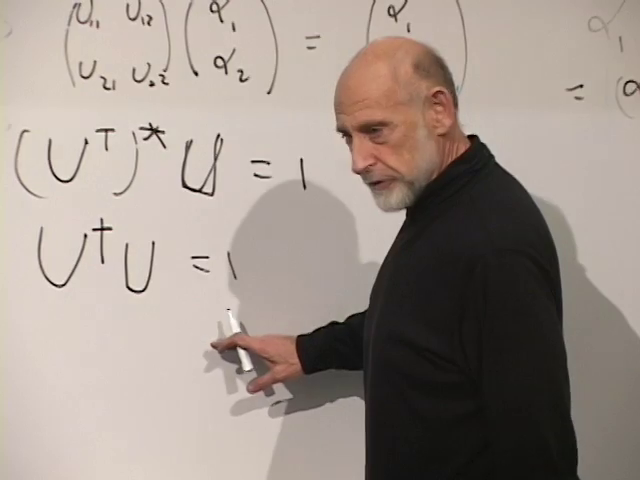
\includegraphics[width=0.62\textwidth]{lecture_03_figure_04.png}
\caption{스피너 회전 행렬은 \(U^\dagger U=\boldsymbol 1\)을 만족한다.}
\lectureframe{00:27:41}
\end{figure}

식~\eqref{eq:l3-unitarity}을 만족하는 행렬은 유니터리 행렬이다. 일반적인 \(2\times2\) 복소 행렬은 실수 매개변수 여덟 개로 시작한다. 유니터리 조건은 \(2\times2\) 행렬 방정식으로, 독립적인 실수 조건 네 개를 제공하므로 매개변수 네 개가 남는다. 공간 회전의 매개변수는 세 개뿐이다. 스피너의 회전 표현을 \(U(2)\) 전체에서 골라내려면 조건이 하나 더 필요하다.

두 열을 복소 벡터 두 개로 보면 조건 네 개를 확인할 수 있다. \(U\)의 각 열은 단위 노름을 가져야 하므로 실수 조건 두 개가 생기고, 두 열은 서로 직교해야 하므로 복소 조건 하나, 즉 실수 조건 두 개가 생긴다. 모두 합해 네 개다. \(U(2)\)에 남은 네 번째 매개변수는 새로운 공간 회전이 아니라 전체 행렬식 위상으로 밝혀질 것이다.

\section{행렬식 1과 \texorpdfstring{\(SU(2)\)}{SU(2)}}

추가 조건은 다음과 같다.
\begin{equation}
\det U=1.
\label{eq:l3-det-one}
\end{equation}
이 조건은 군의 곱셈과 양립한다. 왜냐하면
\begin{equation}
\det(AB)=\det A\,\det B.
\end{equation}
행렬식이 1인 유니터리 행렬 두 개를 곱해도 행렬식은 1이고, 항등행렬의 행렬식도 1이다. 이 행렬들은 닫힌 부분군을 이룬다.

역원도 이 부분군에 속한다. \(\det U=1\)이면 다음과 같다.
\begin{equation}
\det U^{-1}=\frac{1}{\det U}=1.
\end{equation}
따라서 행렬식 1 조건을 부과해도 항등원이 빠지거나 닫힘이 깨지거나 역원이 사라지지 않는다. 이 조건은 연속 매개변수가 하나 적은 군을 일관되게 선택한다.

유니터리 조건만으로도 다음이 성립한다.
\begin{equation}
\det(U^\dagger U)=
(\det U)^*\det U
=|\det U|^2=1.
\end{equation}
하지만 이 조건만으로 \(\det U\)가 \(+1\) 또는 \(-1\)이 되도록 강제되지는 않는다. 일반적인 유니터리 행렬의 행렬식은 임의의 위상일 수 있다.
\begin{equation}
\det U=e^{i\phi},
\qquad
\det U^\dagger=e^{-i\phi}.
\end{equation}
조건~\eqref{eq:l3-det-one}은 이 자유 위상을 고정해 실수 매개변수 하나를 제거한다.

\begin{classroomqa}
\audiencequestion{\(U^\dagger U=\boldsymbol 1\)만으로 \(\det U^\dagger\)가 \(\det U\)와 같거나 오직 \(+1\) 또는 \(-1\)만 되도록 강제되나요?\lecturetimestamp{00:31:21}}
\lecturerresponse{아닙니다. 두 행렬식은 서로 복소켤레입니다. 둘은 \(e^{i\phi}\)와 \(e^{-i\phi}\)일 수 있고, 이들의 곱은 1입니다. 특수 유니터리 조건을 부과하면 두 행렬식 모두 1로 고정됩니다.}
\end{classroomqa}

\(n\times n\) 행렬로 이루어진 유니터리군은 \(U(n)\)이다. \(n=1\)일 때 유니터리 행렬은 위상 \(e^{i\phi}\) 하나이므로 \(U(1)\)이 된다. 행렬식이 1인 부분군은 \emph{특수 유니터리군}이라 하며,
\begin{equation}
SU(n)=\{U\in U(n):\det U=1\}.
\end{equation}
2성분 스피너에는 3매개변수 군인 \(SU(2)\)가 작용한다.

표기법은 두 조건을 모두 나타낸다. \(U\)는 유니터리임을, \(S\)는 특수, 즉 행렬식이 1임을 뜻한다. 특수 유니터리군은 복소 내적을 보존하면서 행렬식에 실리는 독립적인 공통 위상을 배제하므로 여러 곳에서 반복해서 등장한다.

국소적으로 \(SU(2)\)는 스핀 1/2 상태를 회전시키는 데 필요한 회전 대수와 곱셈 구조를 가진다. 전역적으로는 앞서 미룬 세부 사항을 기억해야 한다. \(SU(2)\)는 보통의 회전군 \(SO(3)\)의 이중 덮개이므로, \(SU(2)\)의 원소 두 개가 공간 회전 하나에 대응한다. \editorialnote{이중 덮개라는 정식화는 원문에서 언급만 하고 전개하지 않은 두 겹 대응을 엄밀히 나타낸다.}

\section{무한소 회전과 파울리 행렬}

\begin{classroomqa}
\audiencequestion{스핀 행렬, 즉 파울리 행렬은 이 구성의 어디에서 등장하나요?\lecturetimestamp{00:33:16}}
\lecturerresponse{군 원소를 항등원에 아주 가까이, 즉 회전각이 매우 작은 경우로 두면 등장합니다. 이들은 그런 무한소 회전의 생성자입니다.}
\end{classroomqa}

다음과 같이 두자.
\begin{equation}
U=\boldsymbol 1+\epsilon M+O(\epsilon^2),
\label{eq:l3-small-u-anti}
\end{equation}
여기서 \(\epsilon\)는 실수이며 작다. 그러면
\begin{equation}
U^\dagger=\boldsymbol 1+\epsilon M^\dagger+O(\epsilon^2),
\end{equation}
유니터리 조건으로부터
\begin{align}
U^\dagger U
 &=\boldsymbol 1+\epsilon(M^\dagger+M)+O(\epsilon^2).
\end{align}
1차까지 보면
\begin{equation}
M^\dagger=-M.
\end{equation}
따라서 식~\eqref{eq:l3-small-u-anti}의 행렬 \(M\)은 반에르미트 행렬이다.

여기서는 \(\epsilon\)에 비례하는 항만 남긴다. 곱 \(\epsilon^2M^\dagger M\)은 2차항이므로 버린다. 항등원 가까이에서 다루면 비선형 군 조건이 생성자에 대한 선형 조건으로 바뀐다는 것이 이 방법의 장점이다.

\(i\)를 묶어내는 편이 더 편리하다.
\begin{equation}
U=\boldsymbol 1+i\epsilon H+O(\epsilon^2).
\label{eq:l3-small-u-herm}
\end{equation}
복소켤레를 취하면 \(i\)가 \(-i\)로 바뀌므로
\begin{equation}
U^\dagger=\boldsymbol 1-i\epsilon H^\dagger+O(\epsilon^2).
\end{equation}
이제
\begin{equation}
U^\dagger U
=\boldsymbol 1+i\epsilon(H-H^\dagger)+O(\epsilon^2),
\end{equation}
1차 유니터리 조건은 다음을 요구한다.
\begin{equation}
H^\dagger=H.
\end{equation}
\(i\)를 묶어내면 생성자가 에르미트 행렬이 된다.

\(i\)를 곱해도 허용되는 무한소 행렬은 달라지지 않았다. 생성자에 이름을 붙이는 규약만 달라졌다. 물리학에서는 고유값이 실수이고 각운동량 같은 관측량이 에르미트 연산자이므로 보통 에르미트 생성자를 택한다.

행렬식이 1이라는 조건은 무추적성\editorialnote{말로 행렬식을 전개한 대목에서 첨자가 잠시 잘못 언급되었다. 올바른 선형항은 \(A_{11}+A_{22}=\operatorname{tr}A\)이다. 비대각 원소들의 곱은 2차항부터 나타난다.}을 부과한다. 작은 \(2\times2\) 행렬 \(A\)에 대해
\begin{equation}
\det(\boldsymbol 1+A)
=
\det
\begin{pmatrix}
1+A_{11}&A_{12}\\
A_{21}&1+A_{22}
\end{pmatrix}.
\end{equation}
전개하면
\begin{align}
\det(\boldsymbol 1+A)
 &=(1+A_{11})(1+A_{22})-A_{12}A_{21}\\
 &=1+A_{11}+A_{22}+O(A^2)\\
 &=1+\operatorname{tr}A+O(A^2).
\end{align}
이를 \(A=i\epsilon H\)에 적용하면
\begin{equation}
\det U=1+i\epsilon\,\operatorname{tr}H+O(\epsilon^2).
\end{equation}
따라서 \(\det U=1\)이면 다음을 만족해야 한다.
\begin{equation}
\operatorname{tr}H=0.
\end{equation}
추적 조건은 항등행렬에 비례하는 생성자를 정확히 제거한다. 일반적인 에르미트 \(2\times2\) 행렬에는 실수 대각 성분 두 개와 복소 비대각 성분 하나, 모두 네 개의 실수 매개변수가 있다. 추적 조건은 실수 조합 하나를 고정하므로 세 개가 남는다. 이는 무한소 공간 회전을 할 수 있는 세 축의 개수와 일치한다.

따라서 \(SU(2)\)의 무한소 생성자는 무추적 에르미트 \(2\times2\) 행렬이다. 파울리 행렬 세 개가 기저를 이룬다.
\begin{equation}
\begin{aligned}
\sigma_x&=
\begin{pmatrix}0&1\\1&0\end{pmatrix},
&
\sigma_y&=
\begin{pmatrix}0&-i\\i&0\end{pmatrix},
\\[0.4em]
\sigma_z&=
\begin{pmatrix}1&0\\0&-1\end{pmatrix}.
\end{aligned}
\end{equation}
모든 생성자는 다음과 같이 쓸 수 있다.
\begin{equation}
H=a_x\sigma_x+a_y\sigma_y+a_z\sigma_z.
\end{equation}
\(x\)축을 중심으로 한 작은 회전에는 \(\sigma_x\)가, \(y\)축을 중심으로 한 작은 회전에는 \(\sigma_y\)가 선택된다. 다른 축을 중심으로 회전하면 이에 대응하는 선형결합이 선택된다. \(\hbar=1\)인 단위계에서 스핀 연산자는 다음과 같다.
\begin{equation}
S_i=\frac{\sigma_i}{2}.
\end{equation}

예를 들어 \(x\)축과 \(y\)축의 중간 방향에 해당하는 생성자는 다음에 비례한다.
\begin{equation}
\frac{\sigma_x+\sigma_y}{\sqrt2}.
\end{equation}
계수 벡터의 방향 \((a_x,a_y,a_z)\)가 회전축을 정하고, 그 크기와 \(\epsilon\)가 함께 작은 회전각을 정한다. 이것이 각운동량 교환자에서 등장하는 스핀 행렬과 유한 회전 연산자의 관계다. 특히
\begin{equation}
[S_x,S_y]=iS_z
\end{equation}
그리고 순환적으로 첨자를 바꾼 관계들이 기하학적으로 확인한 비가환성을 나타낸다. 무한소 생성자를 지수화하면 표준적인 유한 회전을 얻는다.\editorialnote{유한 회전의 지수함수 공식은 무한소 구성의 표준적인 완성형이다. 원문에서는 생성자 조건과 파울리 행렬 기저만 유도한다.},
\begin{equation}
U(\hat{\boldsymbol n},\theta)
=\exp\left(-\frac{i\theta}{2}\,
\hat{\boldsymbol n}\cdot\boldsymbol\sigma\right).
\end{equation}
\section{세 상태 색 공간}

표현들을 결합하는 일은 나중에 다루기로 하자. 이제 공간 스핀을 떠나 쿼크의 색으로 돌아간다. 쿼크의 스핀은 여전히 1/2이지만, 색은 그와 독립적인 세 상태 자유도다.
\begin{equation}
\lvert r\rangle,\qquad
\lvert g\rangle,\qquad
\lvert b\rangle.
\end{equation}
일반적인 색 상태는 다음과 같다.
\begin{equation}
\begin{aligned}
\lvert q\rangle_{\mathrm{color}}
={}&
\alpha_r\lvert r\rangle
+\alpha_g\lvert g\rangle
+\alpha_b\lvert b\rangle,
\\
&|\alpha_r|^2+|\alpha_g|^2+|\alpha_b|^2=1.
\end{aligned}
\end{equation}
이를 다음과 같이 쓸 수도 있다.
\begin{equation}
q=
\begin{pmatrix}
\alpha_r\\
\alpha_g\\
\alpha_b
\end{pmatrix}.
\end{equation}
제곱한 절댓값은 선택한 색 기저에서 빨강, 초록, 파랑일 확률이다. 같은 삼중항 표기로 쿼크 장 연산자 세 개를 모아 다음처럼 쓸 수 있다.
\begin{equation}
\psi=
\begin{pmatrix}
\psi_r\\
\psi_g\\
\psi_b
\end{pmatrix}.
\end{equation}

스핀과 색은 개념적으로 구분해야 한다. 스핀 표지는 상태가 물리적 공간의 회전에 어떻게 변환되는지 나타낸다. 색 표지는 실험실을 회전시키지 않는 내부 대칭에 따라 상태가 어떻게 변환되는지 나타낸다. 쿼크 상태는 두 표지를 모두 가지지만, 여기서는 색에 집중하기 위해 스핀은 생략한다.

장 연산자 세 개를 한 열에 쓰는 것은 단순한 정리 방식 이상의 의미가 있다. 이로써 대칭을 하나의 행렬 방정식으로 표현할 수 있다. 공간 회전이 한 벡터 성분을 다른 성분들의 선형결합으로 바꾸듯, 변환에 따라 빨강 장이 빨강, 초록, 파랑 장의 선형결합으로 바뀔 수 있다.

먼저 두 색을 맞바꾸는 이산 변환을 생각해 볼 수 있다. 더 큰 대칭군에는 세 색 모두를 연속적으로 섞는 변환이 포함된다. 단순한 색 교환 행렬은 행렬식이 1이 되도록 위상을 곱해 주어야 할 수 있다. 이렇게 위상을 곱하면 그 교환은 특수 유니터리군 안에 포함된다.

기저 상태 두 개를 그대로 맞바꾸는 변환은 다음 행렬로 나타난다.
\begin{equation}
X=
\begin{pmatrix}0&1\\1&0\end{pmatrix},
\qquad
\det X=-1.
\end{equation}
행렬 전체에 \(i\)를 곱하면 다음을 얻는다.
\begin{equation}
\det(iX)=i^2\det X=1.
\end{equation}
따라서 위상을 일관되게 정하면 이산적인 교환도 더 큰 연속군의 특정 원소로 나타낼 수 있다.

\begin{classroomqa}
\audiencequestion{기저 상태 두 개만 맞바꾸는 행렬은 행렬식이 잘못되어 \(SU(2)\)에 속하지 못하나요?\lecturetimestamp{00:43:46}}
\lecturerresponse{그대로 맞바꾸는 행렬의 행렬식은 \(-1\)입니다. 적절한 \(i\) 인자를 곱하면 행렬식이 1인 대표 원소를 얻을 수 있으므로, 이 교환도 연속적인 특수 유니터리 변환에 포함할 수 있습니다.}
\end{classroomqa}

\section{\texorpdfstring{\(SU(3)\)}{SU(3)}과 여덟 개의 색 생성자}

연속적인 색 변환은 다음과 같다.
\begin{equation}
\begin{aligned}
q'&=Uq,
&
U^\dagger U&=\boldsymbol 1,
\\
\det U&=1,
&
U&\in SU(3).
\end{aligned}
\label{eq:l3-su3-action}
\end{equation}
수학적 구성은 스피너에 사용한 특수 유니터리 구성과 같지만, 이제 \(U\)는 \(3\times3\)이다. 이는 물리적 공간의 회전이 아니다. 내부 색 공간에서의 회전이다.

유니터리 조건은 색 상태의 정규화를 보존한다.
\begin{equation}
q^\dagger q
=|\alpha_r|^2+|\alpha_g|^2+|\alpha_b|^2.
\end{equation}
행렬식 1 조건은 연속적인 혼합에서 공통 \(U(1)\) 위상 방향을 제거한다. 이렇게 얻은 행렬들은 단순한 교환, 상대 위상 변화, 실제로 연속적인 중첩을 만들 수 있으며, 모두 하나의 닫힌 군에 속한다.

매개변수의 개수는 바로 알 수 있다. \(3\times3\) 복소 행렬에는 복소 성분이 아홉 개, 즉 실수 매개변수가 열여덟 개 있다. 행렬 방정식 \(U^\dagger U=\boldsymbol 1\)은 실수 조건 아홉 개를 부과한다. 행렬식 1 조건이 하나를 더 제거한다.
\begin{equation}
\dim SU(3)=18-9-1=8.
\end{equation}
따라서 \(SU(3)\)에는 독립적인 무한소 생성자가 여덟 개 있다.

유니터리 조건의 실수식 아홉 개는 \(U\)의 열을 보면 다시 이해할 수 있다. 복소 열 세 개는 각각 단위 노름을 가져야 하며, 모든 열 쌍은 서로 직교해야 한다. 이 조건들은 처음의 실수 매개변수 열여덟 개 중 아홉 개를 제거한다. 행렬식 위상이 하나를 더 제거해 여덟 개가 남는다. 이는 \(SU(2)\)의 \(8-4-1=3\)와 같은 방식으로 세 상태에 확장한 결과다.

여덟이라는 수가 나타난다는 사실은 결국 글루온 종이 여덟 개가 되는 것과 같은 사실이다. 행렬식 제한으로 한 방향이 제거되었기 때문에 글루온이 아홉 개가 아니라고 말하는 것은 기억을 돕기 위한 표현일 뿐이다. 더 정확히 말하면 아홉 개의 색-반색 행렬은 단위행렬에 비례하는 하나의 색 단일항 방향과 여덟 개의 무대각합 방향으로 분해된다. 이 여덟 무대각합 생성자가 QCD 글루온이 지니는 수반 색 구조를 이룬다.\editorialnote{단일항과 팔중항으로 구성하는 정식화는 원문에서 의도적으로 직관적으로 제시한 행렬식 관련 설명을 엄밀하게 표현한 표준적인 방식이다. 게이지 장의 구성은 뒤에서 다룬다.}

이 단계에서 글루온 여덟 개와의 관계는 앞으로 다룰 내용을 가리킬 뿐, 아직 완전한 유도는 아니다. 게이지 입자를 얻으려면 색 대칭을 국소 대칭으로 승격하고 이를 보상하는 장을 정해야 한다. 매개변수 개수로 이미 밝혀진 것은 \(SU(3)\) 색 변환이 항등원에서 벗어나기 시작할 수 있는 독립적인 방향이 여덟 개라는 점이다.

\section{색 대칭이 QCD를 제약한다}

기본적인 대칭성 진술은 식~\eqref{eq:l3-su3-action}의 색 변환 아래에서 물리가 불변이라는 것이다. 이는 양자색역학의 핵심적인 내부 대칭이다. 색 성분을 섞는 형식은 스핀 위와 스핀 아래의 진폭을 섞는 것과 유사하고, 이러한 스피너 변환은 다시 공간 방향의 회전과 관련되지만, 이 세 공간을 혼동해서는 안 된다.

색을 대칭이라고 하는 것은 색 기저를 바꾸어도 물리적 예측이 달라지지 않는다는 뜻이다. 빨강, 초록, 파랑은 세 기저 벡터를 편의상 부르는 이름이지, 관측 가능한 세 가지 안료가 아니다. 색 성분을 동시에 \(SU(3)\) 회전해도 법칙의 형태는 변하지 않아야 한다. 이 불변성은 선택적인 미적 요소가 아니라 QCD를 조직하는 원리다.

대칭성은 라그랑지안을 제약한다. 앞서 살펴본 \(U(1)\) 예에서는 공통 위상 변환에 대한 불변성으로 인해 장과 그 켤레의 인자가 균형을 이루는 항만 허용되었다. QCD에서도 모든 항은 \(SU(3)\) 색 변환에 대해 불변이어야 한다. 이 요구는 상호작용과 보존량, 글루온 장의 형태에 영향을 준다.

어떤 항이 드러난 색 지수를 가진다고 하자. 식~\eqref{eq:l3-su3-action}에 따르면 그 지수는 회전하므로, 그 항만으로는 불변일 수 없다. 허용되는 항은 색 지수를 불변 조합으로 수축하거나, 변환으로 인한 변화를 보상하는 게이지 장을 사용해야 한다. 이것이 대칭성 원리가 실제로 작용하는 방식이다. 임의의 결합을 배제하고 남는 상호작용을 체계화한다.

QCD를 완성하려면 한 단계가 더 필요하다. 색 변환이 점마다 달라질 수 있어야 하고, 게이지 장은 그 국소적인 변화를 보상해야 한다.\editorialnote{색 대칭을 국소화하는 것은 전역 \(SU(3)\) 대칭성 논의를 게이지 이론으로 완성하는 표준적인 방식이지만, 이 강의 원문에서는 전개하지 않는다.}그 전개는 다음 단계에서 다룬다. 지금은 핵심 구조가 갖추어졌다. 여덟 생성자를 갖는 특수 유니터리 3상태 대칭이 색 삼중항에 작용한다.

당장은 필요한 만큼 군론을 살펴보았다. 일상적인 공간에서 그릴 수 있는 회전에서 시작해 벡터와 스피너에 작용하는 행렬로 나아갔고, 이어 내부 색 공간에서 같은 논리를 다시 사용했다. 이제 수학적 틀을 갖춘 채 입자물리학으로 돌아갈 수 있다. 형식론에 물리적 설명 전체를 한꺼번에 떠맡길 필요는 없다.